\documentclass[a4paper,10pt]{article}

% ------------------------------------
% packages
\usepackage[a4paper,margin=1in,footnotesep=2.2\baselineskip]{geometry}
\usepackage{multicol}
\usepackage{xcolor}
\usepackage{framed}
\usepackage{emoji}
\usepackage[most]{tcolorbox}
\usepackage{fancyhdr}
\usepackage[tracking=true]{microtype}
\usepackage{ragged2e}
\usepackage{listings}
\usepackage{color}
\usepackage{pagecolor}
\usepackage{pdftexcmds}
\usepackage{geometry}
\usepackage{upgreek}
\usepackage{accents}
\usepackage{caption}
\usepackage{bm}
\captionsetup{
  font=small,
  labelfont=bf,
  tableposition=top
}
\usepackage[abspath]{currfile}

\captionsetup[figure]{name=\mono{Figure}}

% ------------------------------------
% checksum = SHA-1
\makeatletter
\ifx\pdf@filemdfivesum\undefined\def\pdf@filemdfivesum#{\mdfivesum file}\fi
\let\filesum\pdf@filemdfivesum
\makeatother

% ------------------------------------
% color definitions
\definecolor{armygreen}{rgb}{0.14, 0.71, 0.15}
\definecolor{darkgreen}{rgb}{0.08, 0.48, 0.18}
\definecolor{darkred}{rgb}{0.86, 0.153, 0.153}
\definecolor{azure}{rgb}{0.0, 0.5, 1.0}
\definecolor{bole}{rgb}{0.82, 0.57, 0.22}
\definecolor{dkgreen}{rgb}{0,0.6,0}
\definecolor{gray}{rgb}{0.5,0.5,0.5}
\definecolor{mauve}{rgb}{0.58,0,0.82}
\definecolor{light-gray}{gray}{0.95}
\definecolor{bg}{HTML}{fcfcfa}
\definecolor{bt}{HTML}{ffebe6}

% ------------------------------------
% code styling
\definecolor{shadecolor}{RGB}{180,180,180}
\newcommand{\code}[1]{\colorbox{shadecolor!30}{\mono{#1}}}
\colorlet{Gray}{gray!20!}
\tcbset{on line, arc=1pt, leftrule=0.25pt,rightrule=0.25pt,toprule=0.25pt,bottomrule=0.25pt,
	boxsep=3pt, left=0pt,right=0pt,top=0pt,bottom=0pt,
	colframe=white,colback=Gray,  
	highlight math style={enhanced}
}
\lstdefinelanguage{Solidity}{
  %keywords={bool, true, false, return, address, bytes32, bytes4, bytes1, bytes, uint256, uint8, uint, string, if, while, else, case, break},
  keywords={},
  keywordstyle=\color{blue}\bfseries,
  %ndkeywords={function,struct, mapping, export, throw, implements, import, this},
  ndkeywords={},
  ndkeywordstyle=\color{darkgreen}\bfseries,
  identifierstyle=\color{black},
  sensitive=false,
  comment=[l]{//},
  morecomment=[s]{/*}{*/},
  commentstyle=\color{green}\mono,
  stringstyle=\color{orange}\mono,
  morestring=[b]',
  morestring=[b]",
  mathescape=true,
  literate={=>}{$\rightarrow{}$}{1}
}
\lstset{
  backgroundcolor=\color{light-gray},
  language=Solidity,
  aboveskip=3mm,
  belowskip=3mm,
  showstringspaces=false,
  columns=flexible,
  basicstyle={\footnotesize\mono},
  numbers=none,
  numberstyle=\tiny\color{gray},
  keywordstyle=\color{blue},
  commentstyle=\color{dkgreen},
  stringstyle=\color{mauve},
  breaklines=true,
  breakatwhitespace=true,
  tabsize=3
}

% ------------------------------------
% fonts
\newfontfamily\pro[Path=./]{__SFMono.ttf}
\newfontfamily\pbold[Path=./]{__SFMonoSemiBold.ttf}
\newfontfamily\mono[Path=./]{__SFMono.ttf}
\newfontfamily\mbold[Path=./]{__SFMonoSemiBold.ttf}
\newfontfamily\robot[Path=./]{__Roboto.ttf}

% ------------------------------------
% heading font-size
\usepackage{sectsty}
\usepackage{fontspec}
\sectionfont{\fontsize{12}{15}\selectfont}
\usepackage[utf8]{inputenc}

% ------------------------------------
% footnote positioning
\usepackage[hang,flushmargin,bottom]{footmisc} 

% ------------------------------------
% bibliography
\usepackage[colorlinks=true,
            linkcolor=blue,
            urlcolor=blue,
            citecolor=blue,
            pdfauthor={sshmatrix},
            pdftitle={Helix2 Protocol},
            pdfsubject={Link Service and Protocol},
            pdfkeywords={ethereum, account, abstraction, link, name, decentralised, distributed},
            pdfproducer={sshmatrix},
            pdfcreator={sshmatrix}]{hyperref}
            
% ------------------------------------
% blank footnote
\newcommand\blfootnote[1]{%
	\begingroup
	\renewcommand\thefootnote{}\footnote{#1}%
	\addtocounter{footnote}{-1}%
	\endgroup
}

% ------------------------------------
% header
\pagestyle{fancy}
\fancyhf{}
\lfoot{\footnotesize \mono{\#}\tcbox{\mono{\filesum{\jobname}}}}
\begin{document}
\setcounter{footnote}{0}
\newpage
\topskip15pt 

\fancyhead[L]{\footnotesize \mono{author}:\tcbox{\mono{sshmatrix}}}
\fancyhead[R]{{\footnotesize \mono{\href{https://github.com/sshmatrix/research}{github.com/sshmatrix/research/zkReview}}}}
\fancyhead[C]{{\footnotesize \emoji{dna}}}
\fancyfoot[C]{{\footnotesize \mono{\thepage}}}
\fancyfoot[R]{{\footnotesize \mono{\today} \emoji{dna}}}

\begin{center}
	\textbf{\Large\pbold{\textls[-40]{Intuitive Interpretation of Non-Interactive Zero-Knowledge Cryptography}}}\\
	\vspace{0.075in}
	\textls[-50]{\mono{A jargon-free approach to understanding zk-SNARKs and zk-STARKs}}\linebreak\linebreak
	\vspace{-0.175in}
	\textls[0]{\mono{Avneet Singh}}\linebreak\linebreak 
	\textls[0]{\mono{SysStruct}}\linebreak
	\textls[0]{\mono{\href{mailto:sshmatrix@pm.me}{sshmatrix@pm.me}}}\linebreak
\end{center}
\begin{center}
	\textbf{\Large\pbold{ABSTRACT}}\linebreak\linebreak
	\textls[-50]{\mono{zk-SNARKs and zk-STARKs are relatively new concepts in cryptography, yet they are being touted as the next forefront in modern and future crypto tech. In blockchain space specifically, there is great interest in these subfields in context of zk-Rollups to Layer 1 blockchains such as Ethereum, or as standalone decentralised ledgers with high rates of transactions per second (TPS), e.g. Aztec Network (zk-STARK), zkSync, Loopring, ZCash (zk-SNARKs) etc. Despite their great importance in cryptography, it is unfortunately difficult to understand zk-SNARKs and zk-STARKs due to limited literature and conceivably difficult mathematics conveyed through intensive jargon. This paper is an attempt to introduce zero-knowledge (zk) cryptography in an intuitive manner to garden-variety mathematicians, physicists, curious blockchain developers and perhaps even cryptographers.}}
\end{center}
\vspace{0.2in}
\begin{flushleft}
	\textbf{\Large\pbold{INTRODUCTION}}\linebreak\linebreak
	\textls[-50]{\mono{Zero-knowledge cryptography (ZKC) is presumably the next natural step in cryptography's evolution toward post-quantum era. zk-SNARKs and zk-STARKs are specific implementations of zero-knowledge cryptography that are widely considered the most promising paths toward post-quantum security. In order to deeply understand zero-knowledge cryptography, one must at least understand the current generation cryptographic systems such as RSA (Rivest–Shamir–Adleman) and Elliptic Curve Cryptography (ECC); this is admittingly a challenging task since the mathematics of such protocols is rather tedious and it only gets worse as one ventures into zero-knowledge protocols. Despite these challenges, it is nevertheless easier to understand at least the philosophy and intuition behind zero-knowledge protocols using the famous Alibaba Cave example [1] without requiring any prerequisite knowledge of RSA or ECC. We leave this as an exercise for the reader. In this paper, we will attempt to delve into the practical implementation of zero-knowledge protocols while retaining an intuitive understanding of the underlying mathematical processes.\linebreak\linebreak
	}}
	\colorbox{Gray}{\hspace{1mm}\parbox{0.99\textwidth}{\vspace{1mm}\textls[-50]{\mono{Through the course of this paper, additional comments in a grey box should be interpreted are anecdotes, comparisons or similariries that may help readers develop an intuitive understanding. In addition, we encourage readers to read this paper in conjunction with [10].\vspace{1mm}}}}}
\end{flushleft}
\begin{flushleft}
	\textls[-50]{\mono{Cryptographic protocols at their core are motivated by the need to prove access to some information without necessarily revealing a part or the entirety of said information. In mathematical terms, there are several ways of achieving this functionality from an intelligently designed system.\linebreak
	}}
\end{flushleft}
\begin{flushleft}
	\textbf{\large\pbold{PRIME NUMBERS}}\linebreak\linebreak
	\textls[-50]{\mono{Cryptographers realised back in the day that prime numbers were one such system that could provide the desired functionality. For instance, consider two sufficiently large prime numbers {\upalpha} = 53781811 and {\upgamma} = 23252729, and their even larger product {\upalpha}\bm{$\;\times\;$}{\upgamma} = 1250573876312219. The product 1250573876312219 is a relatively difficult number to prime factorise back to {\upalpha} and {\upgamma} if both {\upalpha} and {\upgamma} are unknown. However, if either one of the two prime factors ({\upalpha} or {\upgamma}) are known, then it is straightforward to calculate the other unknown prime factor by simple division. To intuitively understand this system further, let's break it down into its principle components: we took a set of very large prime numbers of which {\upalpha} and {\upgamma} are members and defined an operation of product\textsuperscript{\textcolor{blue}{1}}\blfootnote{\textls[-50]{\mono{\textsuperscript{1}The operations of addition '+' and its inverse subtraction '-' are implictly defined}}} on the members of the set; such a finite field is called a Galois field. Additionally, we note that the product operation \bm{$\times$} is difficult to invert unless one of the two numbers is known; this kind of a system is usually called a trapdoor. Trigonometric functions like sine({\upalpha}) in real space and e\textsuperscript{i\upalpha} in complex space are some other naive examples of trapdoors.\linebreak\linebreak 
	}}
	\colorbox{Gray}{\hspace{1mm}\parbox{1.0\textwidth}{\vspace{1mm}\textls[-50]{\mono{In abstract mathematics, such a system is called a Group and the study of groups is called Group theory; a group is defined by a set of elements (called a Field, e.g. large prime numbers) along with the set of permitted operations between those elements (e.g. product). The configuration of any trapdoor system is such that the permitted operations defined on the elements of the group are difficult to invert.\vspace{1mm}}}}}\linebreak\linebreak\linebreak
	\textbf{\Large\pbold{RSA CRYPTOGRAPHY}}\linebreak\linebreak
	\textls[-50]{\mono{RSA protocol is one of the simplest implementations of the trapdoor feature which results in a keypair system - a public key and a private/secret key - typically utilised in conjunction for encrypting and decrypting information. The premise of the RSA protocol essentially lies in setting, i) public key as the qualitative equivalent of the product {\upalpha}\bm{$\;\times\;$}{\upgamma}, and ii) private key as the qualitative equivalent of either {\upalpha} or {\upgamma}, where {\upalpha} and {\upgamma} are restricted to a finite field of prime numbers. The security of such a system is encoded in the difficulty of prime factorising the product. It is unimportant to know the precise details of the protocol implementation in context of this paper. In nutshell, the RSA algorithm requires solving for the integer coefficients (x,\,y) of Bezout's Identity x\,\cdot\,{\upalpha} + y\,\cdot\,{\upgamma} = 1 using extended Euclidean algorithm [2] and employing modular arithmetic to wrap integer numbers when they fall outside the range of a separately defined composite finite field F\textsubscript{\pbold{p'}}.\linebreak\linebreak
	}}
	\colorbox{Gray}{\hspace{1mm}\parbox{1.0\textwidth}{\vspace{1mm}\textls[-50]{\mono{Modular arithmetic is quite simply equivalent to applying the modulo '\%' operation over some prime number {\pbold{p}} to all group operations $\bullet$ (i.e. $\bullet$ = \bm{$+$}, $-$, \bm{$\times$} or $/$), such that {\upalpha} $\bullet$ {\upgamma} $\rightarrow$ {\upalpha} $\bullet$ {\upgamma} \% {\pbold{p}}. Modular airthmetic is regular arithmetic 'wrapped' by the modulo operator such that results of all group operations lie within 0 and {\pbold{p}}; the range of \% {\pbold{p}} is called a prime field F\textsubscript{\pbold{p}}. For example, new operations are: {\upalpha} \bm{$+$} {\upgamma} $\rightarrow$ ({\upalpha} \bm{$+$} {\upgamma}) \% {\pbold{p}}, {\upalpha} $-$ {\upgamma} $\rightarrow$ ({\upalpha} $-$ {\upgamma}) \% {\pbold{p}}, {\upalpha} \bm{$\times$} {\upgamma} $\rightarrow$ ({\upalpha} \bm{$\times$} {\upgamma}) \% {\pbold{p}} and most notable, {\upalpha} $/$ {\upgamma} $\rightarrow$ ({\upalpha} \bm{$\times$} {\upgamma}\textsuperscript{{\,\pbold{p}} - 2}) \% {\pbold{p}}.\vspace{1mm}}}}}\linebreak\linebreak\linebreak
	\textbf{\large\pbold{ROBUSTNESS OF RSA}}\linebreak\linebreak
	\textls[-50]{\mono{While RSA is sufficiently safe to use today, it's safety will decrease over time as computational capacity of human civilisation increases. This is because the fastest and - arguably - maximally efficient algorithms capable of inverting the {\upalpha}\bm{$\;\times\;$}{\upgamma} product are iterative by construction and rely on optimised brute-forcing; Quadratic Sieve [3] and General Number Field Sieve [4] are two such well-known methods. With the advent of quantum computers, RSA algorithm's security will be definitively compromised; this is the so called SNDL problem (Save-Now-Decrypt-Later) facing the cryptography community today [5]. The core issue at hand here is that prime finite fields (meaning finite field of prime numbers; not to be confused with a prime field) and the generic operation of product on them - irrespective of the largeness of its elements - does not possess sufficient difficulty if the exploitor has relatively large computational resources at hand. In order to design better cryptosystems that are secure against brute-forcing, one must come with a new group with a better choice of finite field and a preferably a harder group operation which is resistant to such an attack.\linebreak\linebreak\linebreak
	}}
	\textbf{\Large\pbold{DIFFIE-HELLMAN KEY EXCHANGE}}\linebreak\linebreak
	\textls[-50]{\mono{In very few lines, let us discuss the Diffie-Hellman Key Sharing Algorithm. Unlike RSA which is a keypair-based algorithm with a public key identity, Diffie-Hellman is a 'secret sharing' method between two parties who each possess a secret private key and a shared public key. Diffie-Hellman in some sense is the intermediate step between RSA and ECC since it introduces relatively simple finite fields over groups other than itself; this simply means that instead of explicitly operating on a set of prime numbers (e.g. in RSA), we will instead operate on 'cyclic' functions of primes {\pbold{C}}({\pbold{p}}).\linebreak\linebreak
	}}
	\colorbox{Gray}{\hspace{1mm}\parbox{1.0\textwidth}{\vspace{1mm}\textls[-50]{\mono{In a finite cyclic group with N elements (i.e. of "order" N), all N elements can be derived by repeatedly performing the group operation on one of the elements (called the generator). We can thus represent the K-th element in such a group with notation {\pbold{G}}\textsuperscript{K}, representing K group operations on the generator element {\pbold{G}}; note that the term {\pbold{G}}\textsuperscript{K} should not be interpreted as a literal exponent although a lot of literature uses this terminology. The use of exponential notation results from the classical Diffie-Hellman algorithm using the literal exponent of a 'primitive root modulo {\pbold{p}}', i.e. G = G\textsuperscript{K} as the group operation on prime finite fields, i.e. {\pbold{G}}\textsuperscript{K} $\equiv$ (G \bm{$\times$} G \bm{$\times$} G \bm{$\times$} G \bm{$\times$}\,{\cdot\cdot\cdot}\, \bm{$\times$} G)\textsubscript{K = 0,\,1,\,2,\,3\,\;{\cdot\cdot\cdot}\,\;(N - 1)}. The final form of {\pbold{C}}({\pbold{p}}) thus reads {\pbold{G}}\textsuperscript{K} \% {\pbold{p}}. The cyclicity of e\textsuperscript{i\pbold{z}} in complex space is another reason for the exponential notation.\vspace{1mm}}}}}\linebreak\linebreak\linebreak
	\textls[-50]{\mono{In practise, the private key for two parties is derived by evaluating the function {\pbold{C}}({\pbold{p}}) = {\pbold{G}}\textsuperscript{K} \% {\pbold{p}} from commonly known values of {\pbold{G}} and {\pbold{p}} at two values of K = {\upmu},\,{\upnu}. The shared key then takes the form of {\pbold{G}}\textsuperscript{\upmu\upnu} \% {\pbold{p}}, which is also the non-invertible term securing the protocol\textsuperscript{\textcolor{blue}{2}}\blfootnote{\textls[-50]{\mono{\textsuperscript{2}{Note that {\upmu} and {\upnu} are not necessarily prime numbers}}}} instead of a simple product between two large prime numbers. Breaking the Diffie-Hellman method is thereby different from RSA since it involves inverting {\pbold{G}}\textsuperscript{\upmu\upnu} \% {\pbold{p}} instead of {\upalpha}\bm{$\;\times\;$}{\upgamma}; this is known as the Computational Diffie-Hellman Problem (C-DHP).\linebreak\linebreak
	}}
	\colorbox{Gray}{\hspace{1mm}\parbox{1.0\textwidth}{\vspace{1mm}\textls[-50]{\mono{More specifically, C-DHP states that given the knowledge of {\pbold{G}}\textsuperscript{\upmu} and {\pbold{G}}\textsuperscript{\upnu} (but not {\upmu} and {\upnu}), it is difficult to compute the value of {\pbold{G}}\textsuperscript{\upmu\upnu}. More simply, if we are revealed the values of two elements derived from secretly taking \upmu} and {\upnu} cyclic operations, then it is difficult to compute the element derived by taking {\upmu}\bm{$\;\times\;$}{\upnu} cyclic operations. One variant of Diffie-Hellman problem which is easy to solve in this case is the Decisional Diffei-Hellman Problem (D-DHP). D-DHP states that given knowledge of three elements {\pbold{G}}\textsuperscript{\upmu}, {\pbold{G}}\textsuperscript{\upnu} and {\pbold{G}}\textsuperscript{\upsigma} (but not {\upmu}, {\upnu} or {\upsigma}), it is probabilistically easy to determine whether {\pbold{G}}\textsuperscript{\upmu\upnu} = {\pbold{G}}\textsuperscript{\upsigma}. In other words,\vspace{1mm}}}}\linebreak
	\colorbox{Gray}{\hspace{1mm}\parbox{1.0\textwidth}{\vspace{1mm}\textls[-50]{\mono{given {\pbold{G}}\textsuperscript{\upmu} and {\pbold{G}}\textsuperscript{\upnu}, while it is hard to determine {\pbold{G}}\textsuperscript{\upmu\upnu}, it is relatively easier to determine whether a third randomly chosen element {\pbold{G}}\textsuperscript{\upsigma} is a result of {\pbold{G}}\textsuperscript{\upmu\upnu}. While the relative ease of solving D-DHP may not be obvious, the proof of it becomes apparent after taking into account the Law of Quadratic Reciprocity of Legendre symbols [9]; this however falls out of scope of this paper.\vspace{1mm}}}}}\linebreak\linebreak\linebreak
	\textbf{\Large\pbold{ELLIPTIC CURVE CRYPTOGRAPHY}}\linebreak\linebreak
	\textls[-50]{\mono{The fundamental issue that leads to the breakdown of RSA algorithm is that the prime number field and the operation of product is not complex enough in the face of large computational power. The effort to improve on this problem led to the advent of Elliptic Curve Cryptography (ECC). ECC functions by fixing the core illnesses in RSA, i.e. it proposes - similar to Diffie-Hellman - that instead of operating on the prime number field itself, we operate on another field on which we define a newer set of operations that are much harder to invert. The premise of ECC thus lies in the introduction of prime finite fields over special elliptic curves, a step up from simple cyclic groups used in Diffie-Hellman [7]. In context of cryptography, an Elliptic curve is simply the following relation between a prime finite field {\pbold{x}} and composite field {\pbold{y}},
	}}
	\vspace{2mm}
	\begin{center}
		{\mono{{\pbold{y}}\textsuperscript{2} = {\pbold{x}}\textsuperscript{3} + g\textsubscript{1}\,\cdot\,{\pbold{x}} + g\textsubscript{2}, \\
		\vspace{2mm}
		\textls[-50]{\mono{given}} 4\,g\textsubscript{\textsubscript{\scriptsize{1}}}\hspace{-1.8mm}\textsuperscript{3} + 27\,g\textsubscript{\textsubscript{\scriptsize{2}}}\hspace{-1.8mm}\textsuperscript{2} {\robot{^^^^2260}} 0
		}}
	\end{center}
	\begin{flushright}
		{\vspace{-7.5mm}\mono{(1)}}
	\end{flushright}
	\vspace{2mm}
	\textls[-50]{\mono{Gigabrains realised few decades ago that the elliptic curves have some very cool properties in context of invertibile binary operations. To begin with,
	\linebreak
	}}
\end{flushleft}
\begin{multicols}{2}
	\noindent
	\begin{minipage}{\linewidth}
		\centering
		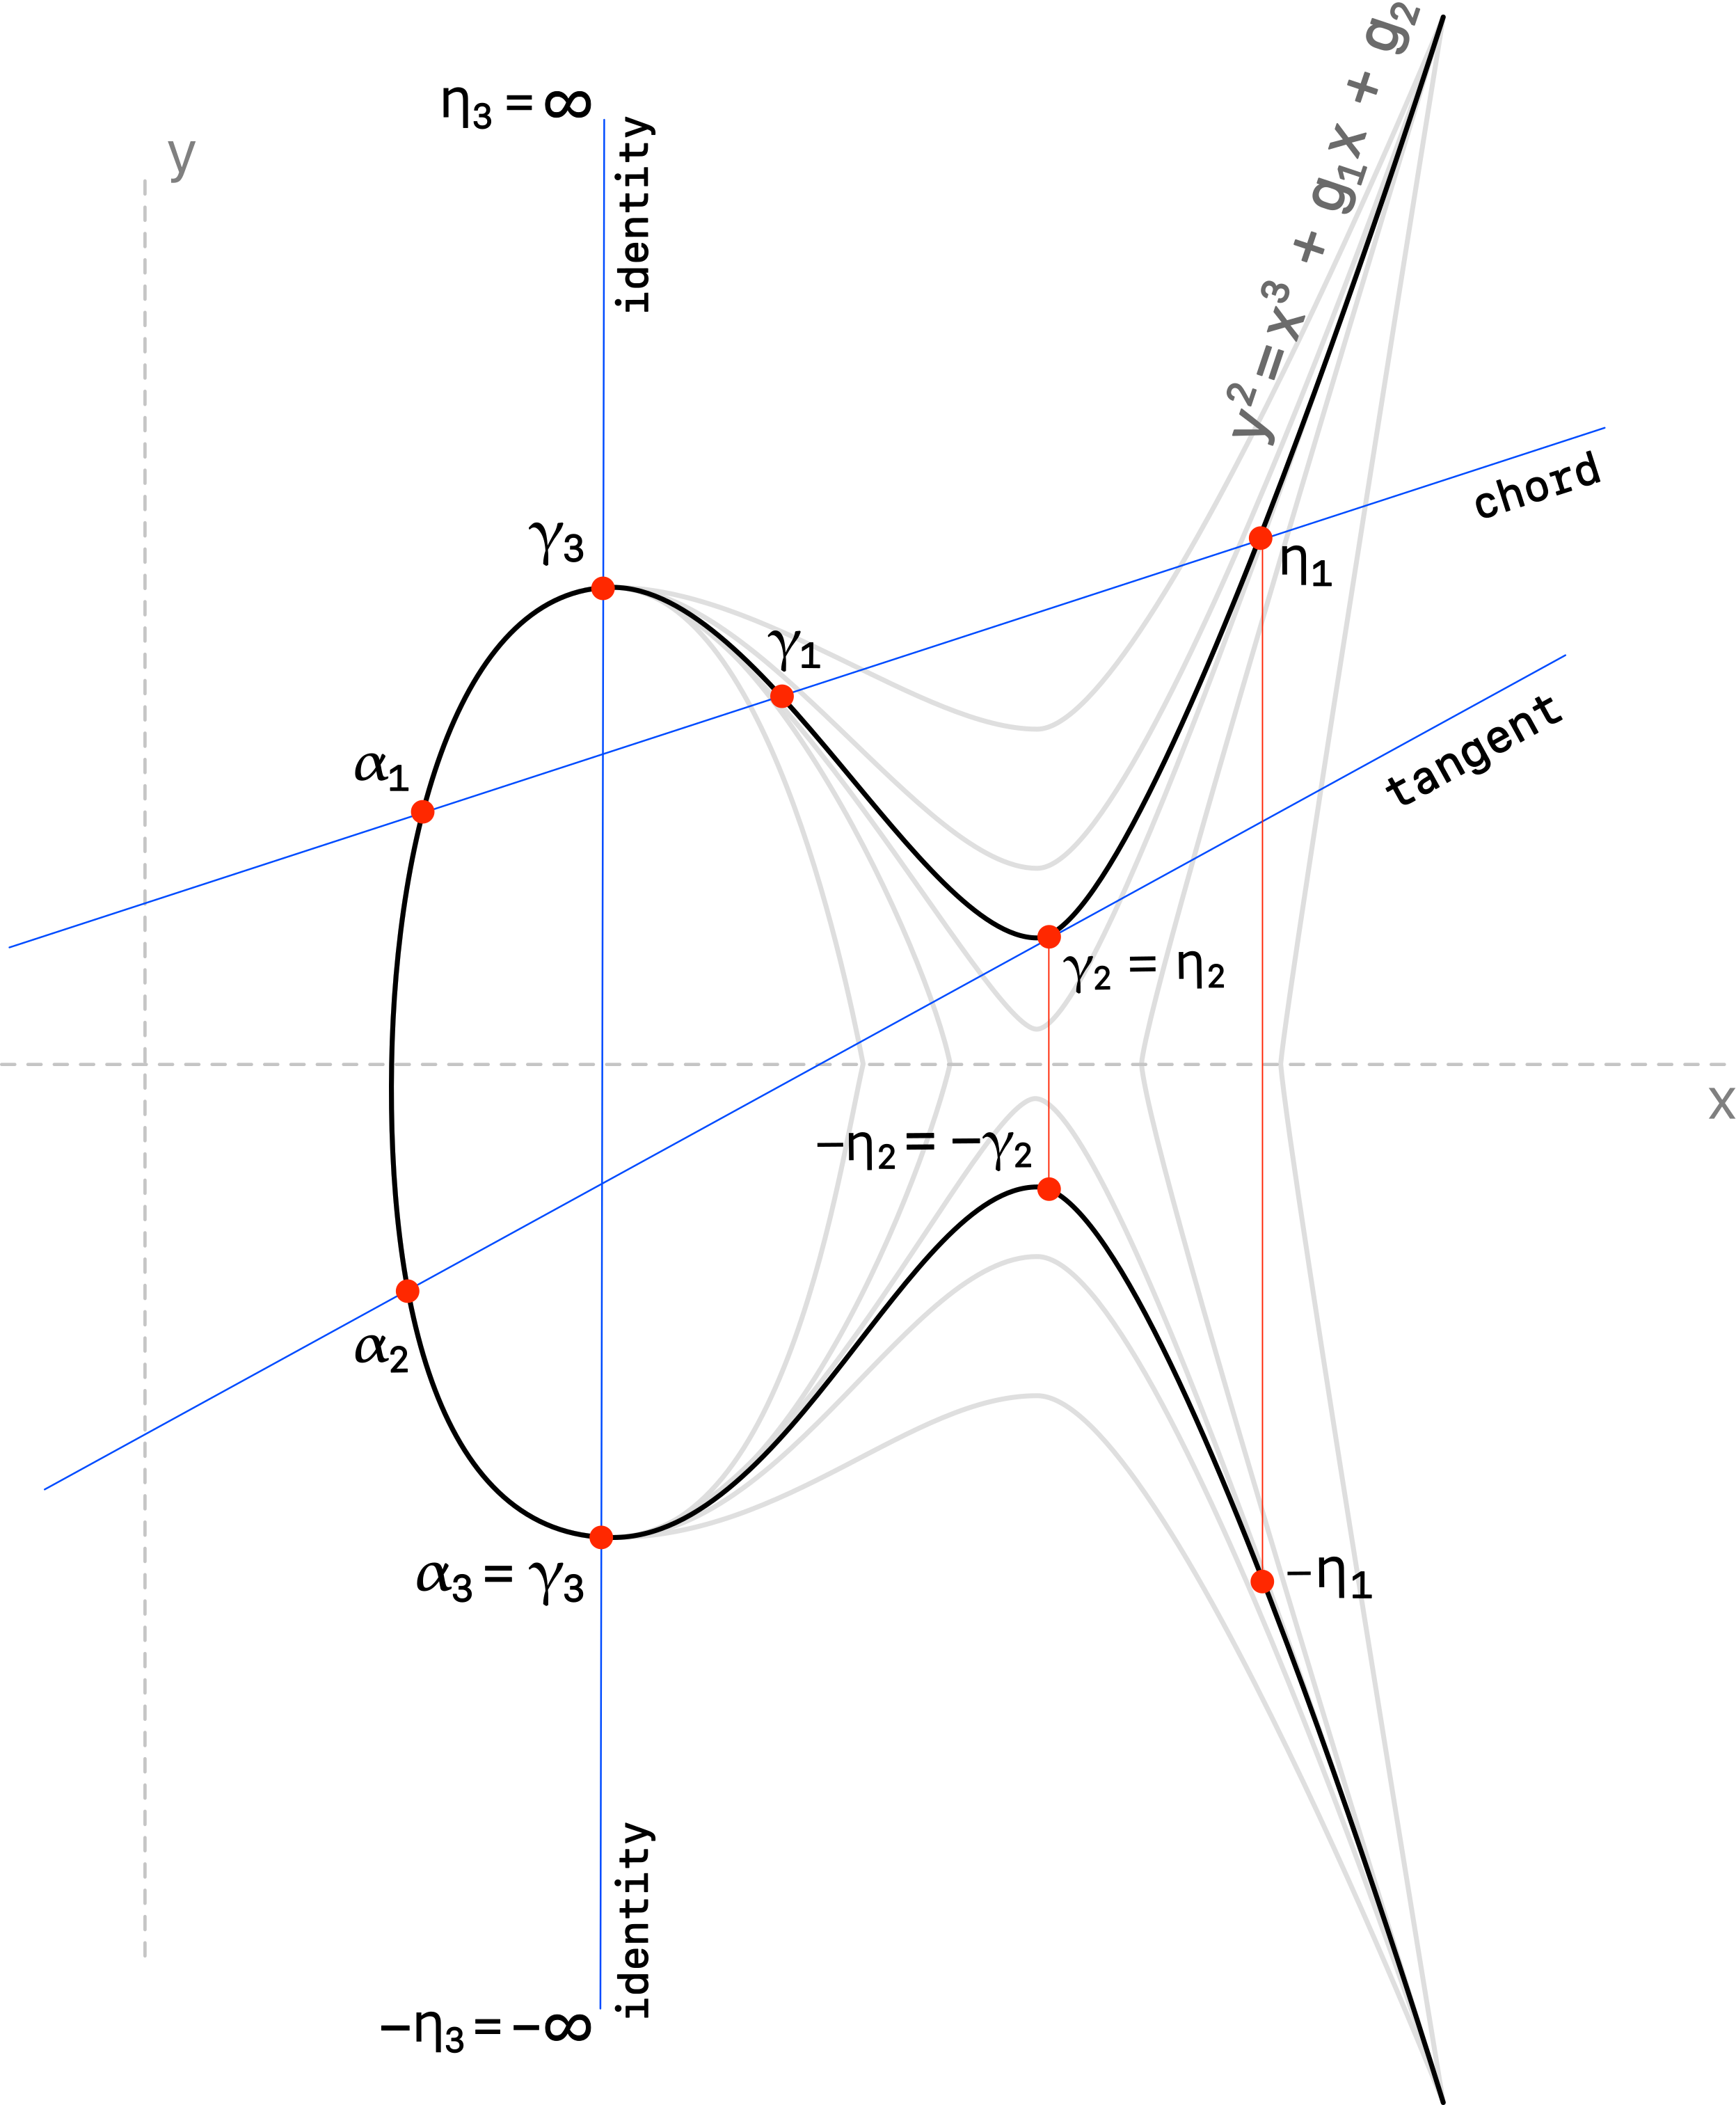
\includegraphics[width=80.68mm]{./img/ellipticCurve.png}
		\captionof{figure}{\textls[-50]{\mono{Elliptic curve over a continuous infinite field, aka a Lie group. We ignore the finite field contraint in this figure for simplicity. Three examples are shown depicting how to interpret different intersectionsof the line with the elliptic curve and the infinity point.}}}
		\label{fig:ecc0}
	\end{minipage}
	\noindent
	\begin{minipage}{\linewidth}
		\centering
		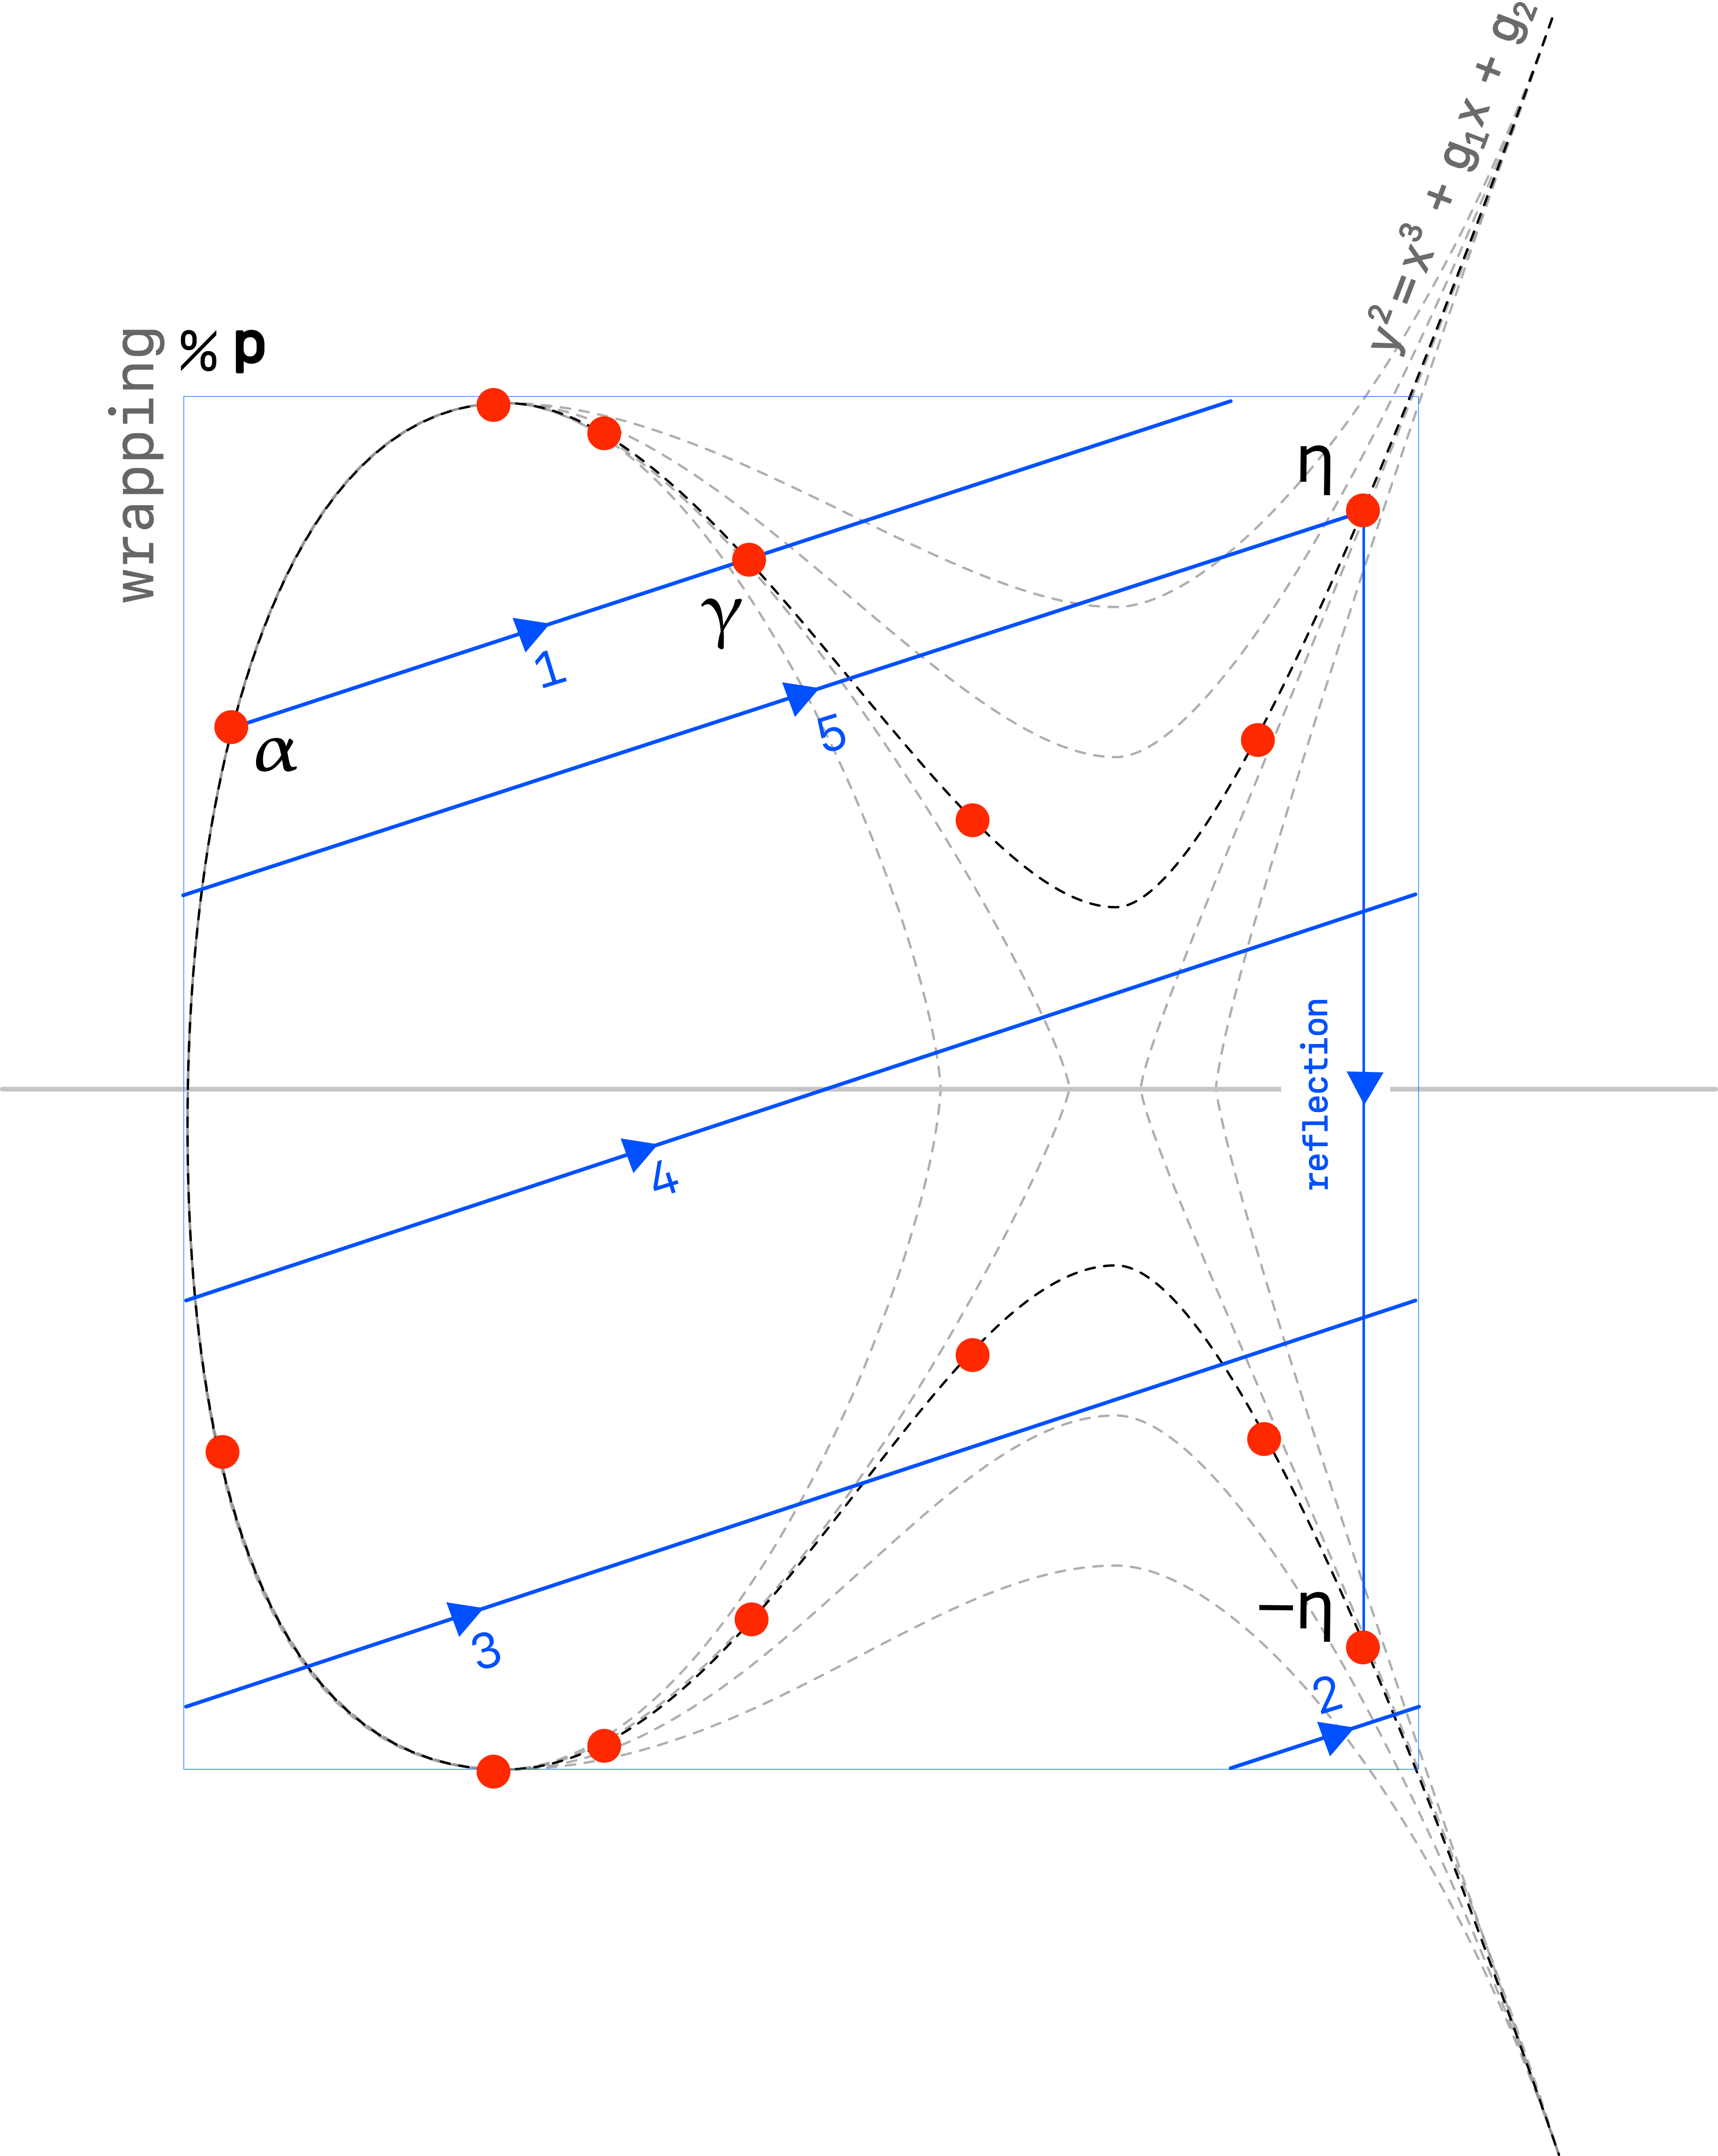
\includegraphics[width=78mm]{./img/ECC.png}\vspace{-0.1mm}
		\captionof{figure}{\textls[-50]{\mono{Example elliptic curve evaluation over a prime finite field modulo {\pbold{p}}; the effect of the modulo operator \% is to "wrap" the out-of-range values to within range. In the above example, it takes 5 'wrappings' and 1 final reflection to calculate -{\,\upeta}.}}}
		\label{fig:ecc1}
	\end{minipage}
\end{multicols}
\begin{flushleft}
	\textls[-50]{\mono{1. The elliptic curve is symmetric across the x-axis; this is desirable since it ensures existence of both {\pbold{y}} and -{\pbold{y}} in our group. More importantly,\linebreak\linebreak
	2. For any two points {\upalpha} and {\upgamma} on the elliptic curve, a line through them intersects the elliptic curve again at most - but not necessarily - 1 more point, denoted by {\upeta}; the blue line in figure \ref{fig:ecc0} is one such example.\linebreak\linebreak
	}}
	\textls[-50]{\mono{Typically, {\pbold{x}} is taken as the independent prime finite field and {\pbold{y}} is the so-called 'elliptic curve (evaluation) over finite field'; {\pbold{y}} are the elements of our desired new group. Ignoring the finite field constraint for a moment, the elliptic curve is shown in figure \ref{fig:ecc0} when {\pbold{x}} is a continuous real variable. Our task now is to come up a hard-to-invert group operation on the continuous elements {\pbold{y}} of our new group; we will reinstate the prime finite field constraint afterwards.
	}}
	\textls[-50]{\mono{Note that it is possible for the line to not intersect the curve for the third time at all, and these singularities are in fact necessary for our group to function. Consider, the green line in figure \ref{fig:ecc0}; note that all vertical lines intersect the curve at exactly two points. It is also possible for a tangent to the curve to intersect the curve at exactly two points; see one such example (the red line) in figure \ref{fig:ecc0}. The aforementioned gigabrains soon realised that one can use this intersectional property of a line with the elliptic curve (aka properties 1. and 2.) as the new group operation \bm{$\oplus$} such that
	}}
	\begin{center}
		\mono{{\upalpha} \bm{$\oplus$} {\upgamma} =\;\,-{\,\upeta}}
	\end{center}
	\begin{flushright}
		{\vspace{-7mm}\mono{(2)}}
	\end{flushright}
	\textls[-50]{\mono{This is the same as saying that \bm{$\oplus$} operation between {\upalpha} and {\upgamma} is equivalent to taking reflection (-) of the third intersection point {\upeta} across x-axis. Most literature phrases this \bm{$\oplus$} operation as the new "addition" operation on the group elements of {\pbold{y}}. However, we noted before that the third intersection {\upeta} doesn't exist for all pairs {\upalpha} and {\upgamma}; in jargon-speak, we say that 'the group is not closed under the \bm{$\oplus$} operation'.
	}}
	\textls[-50]{\mono{We can solve this closeness problem by explicitely including the infinity element {\robot{^^^^221e}} to the group. Once we have access to {\robot{^^^^221e}}, all intersections similar to the green line are assumed to intersect the curve again at {\upeta} = {\robot{^^^^221e}}, such that
	}}
	\begin{center}
		\mono{{\upalpha} \bm{$\oplus$} {\robot{^^^^221e}} = {\upalpha}}
	\end{center}
	\begin{flushright}
		{\vspace{-7mm}\mono{(3)}}
	\end{flushright}
\end{flushleft}
\begin{flushleft}
	\textls[-50]{\mono{Note that {\robot{^^^^221e}} acts like the identity element \^I of our new group since it satisfies {\upalpha} \bm{$\oplus$} \^I = {\upalpha}. Lastly, the third case of the red line is not difficult since it is simply a special case of the blue line when {\upgamma} = {\upeta}; another important tangent case arises when {\upalpha} = {\upgamma}, such that {\upalpha} \bm{$\oplus$} {\upalpha} = {\upeta}. Now we have all the ingredients required to construct a robust inverse problem on our new group {\pbold{y}} with the permitted operation \bm{$\oplus$}. We reinstate the requirement of evaluating the elliptic curve on a prime finite field by explicitely defining a finite field range and wrapping the out-of-range evaluations over the elliptic curve with the modulo operator \% {\pbold{p}}. The final form of the \bm{$\oplus$} operation is shown in figure \ref{fig:ecc1}. In a real world ECC implementation, this process is carried out a large number of times (assuming {\upalpha} = {\upgamma}, i.e. take tanget at point {\upalpha}) making the forward process increasingly complex but computable and the resulting inverse problem increasingly difficult to solve.\linebreak\linebreak
	}}
	\colorbox{Gray}{\hspace{1mm}\parbox{1.0\textwidth}{\vspace{1mm}\textls[-50]{\mono{In literature, you will often find the operation \bm{$\oplus$} equated to the generic addition \bm{$+$}. This is not surprising since equations (2) and (3) resemble a + b = c and a + 0 = a for generic real numbers; 0 is the identity element of the \bm{$+$} operation. Having said that, in practice \bm{$\oplus$} operation is nothing like the addition operation \bm{$+$}; the apparent similarity lies in their algebraic representations only. For instance, equations (2) and (3) also resemble a \bm{$\times$} b = c and a \bm{$\times$} 1 = a for generic real numbers. In this case, 1 is the identity element of the \bm{$\times$} operation.\vspace{1mm}}}}}\linebreak
	\textls[-50]{\mono{The 'large number of repetitions' is assigned as the secret private key K\textsubscript{sec} and the public key K\textsubscript{pub} is equivalent to calculating {\upalpha} \bm{$\oplus$} {\upalpha} at a public value {\upalpha} = {\upalpha}\textsubscript{o} repeated K number of times\textsuperscript{\textcolor{blue}{3}}\blfootnote{\textls[-50]{\mono{\textsuperscript{3}{\upalpha} = {\upgamma} assertion is made purely for simplicity since having {\upalpha} {\robot{^^^^2260}}\;\,{\upgamma} doesn't provide extra security and in fact makes the forward computation unnecessarily require two generator elements.}}}, i.e. K\textsubscript{pub} = (\,{\cdot\cdot\cdot}\,(({\upalpha}\textsubscript{o} \bm{$\oplus$} {\upalpha}\textsubscript{o})\textsubscript{1} \bm{$\oplus$} {\upalpha}\textsubscript{o})\textsubscript{2} \bm{$\oplus$} {\upalpha}\textsubscript{o})\textsubscript{3}\,{\cdot\cdot\cdot}\,)\textsubscript{K}. The exact inverse problem - called the Discrete Logarithm Problem (DLP) - is equivalent to finding the number of repetitions it took to arrive at K\textsubscript{pub} from a publicly known value {\upalpha}\textsubscript{o}. Is this inverse problem hard? It appears that given knowledge of K\textsubscript{pub} and {\upalpha}\textsubscript{o}, one can easily revert the process described in figure \ref{fig:ecc1} and derive key K\textsubscript{sec}. This is indeed true and the inverse problem only becomes hard when the coefficients in equation (1) are restricted to a finite field of large primes; more on this in the next subsection. Some of the popular elliptic curves today are specifically \code{ed25519} and \code{secp256k1}, with the later being more recent and more robust than the former.\linebreak\linebreak
	}}
	\colorbox{Gray}{\hspace{1mm}\parbox{1.0\textwidth}{\vspace{1mm}\textls[-50]{\mono{The name of the inverse problem for ECC, i.e. discrete logarithm problem (DLP), is highly misleading and results from purely notational reasons. The term 'logarithm' originates from interpreting the result of K times repetition of {\upalpha} \bm{$\oplus$} {\upalpha} operation such that K\textsubscript{pub} = {\upalpha}\textsuperscript{K}.\vspace{1mm}}}}}\linebreak\linebreak\linebreak
	 \textls[-50]{\mono{It now appears that we have achieved what we set out to do: we have found a new group who elements are now {\pbold{y}} in prime field F\textsubscript{\pbold{p}} evaluated over the prime finite field and the new group operation (\,{\cdot\cdot\cdot}\,(({\upalpha}\textsubscript{o} \bm{$\oplus$} {\upalpha}\textsubscript{o})\textsubscript{1} \bm{$\oplus$} {\upalpha}\textsubscript{o})\textsubscript{2} \bm{$\oplus$} {\upalpha}\textsubscript{o})\textsubscript{3}\,{\cdot\cdot\cdot}\,)\textsubscript{K} $\equiv$ {\upalpha}\textsubscript{\,o}\hspace{-2.1mm}\textsuperscript{\,K} is very difficult to invert. We note that the result of \bm{$\oplus$} operation on the group elements results in a value which is also a member of the group\textsuperscript{\textcolor{blue}{4}}\blfootnote{\textls[-50]{\mono{\textsuperscript{4}The group is referred to as 'closed under the operation \bm{$\oplus$}'}}}; this was not the case in RSA scheme where the result {$\upalpha$}\bm{$\;\times\;$}{\upgamma} is never a member of the group.\linebreak\linebreak
	}}
	\textls[-50]{\mono{Curious observers may note that unlike RSA where we keep both {\upalpha} and {\upgamma} secret (and reveal their product {\upalpha}\bm{$\;\times\;$}{\upgamma}), in ECC we additionally also reveal one of the independent variables {\upalpha}\textsubscript{o}, i.e. {\upalpha}\textsubscript{\,o}\hspace{-2.1mm}\textsuperscript{\,K} and {\upalpha}\textsubscript{o} are both known, leaving only K to be discovered. Why is this the case? The answer lies in the fact that the solutions {\upalpha} and {\upgamma} of the product {\upalpha}\bm{$\;\times\;$}{\upgamma} are unique while the solutions {\upalpha} and K of the expression {\upalpha}\textsuperscript{K} are not unique unless either {\upalpha} or K is specified. Uniqueness of the keypairs is a very important property that cannot be violated for cryptosystems; this requires {\upalpha}\textsubscript{o} to be fixed and specified publicly in ECC algorithms.\linebreak\linebreak
	}}
	\textls[-50]{\mono{Curious observers may additionally note that the expression {\upalpha}\textsuperscript{K} looks very similar to the {\pbold{G}}\textsuperscript{K} expression in Diffie-Hellman. How similar are these two? Quite a lot actually. The group defined by {\upalpha}\textsuperscript{K} is in fact also a finite cyclic group with {\upalpha}\textsubscript{o} as its generator element! The order N, i.e. number of elements in the group, is defined by the expression {\upalpha}\textsubscript{\,o}\hspace{-2mm}\textsuperscript{\,N} = \^I = {\robot{^^^^221e}}. Does this mean we can construct an even safer Diffie-Hellman Key Sharing algorithm by using an elliptic curve to construct the cyclic field instead of the simple choice made in classical Diffie-Hellman? The answer is yes we can and such methods already exist in the form of Elliptic Curve Diffie-Hellman algorithms [8].\linebreak\linebreak
	}}
	\textbf{\large\pbold{ROBUSTNESS OF ECC}}\linebreak\linebreak
	\textls[-50]{\mono{The natural question to ask here is: how robust is ECC when compared to RSA and Diffie-Hellman? We remember from previous section that the inverse problem in ECC only becomes hard when the coefficients p and q in equation (1) are also restricted to a finite field of large primes. To understand why this happens, simply note that for large prime values of g\textsubscript{\textsubscript{\scriptsize{1}}}, g\textsubscript{\textsubscript{\scriptsize{2}}} and {\pbold{x}} in equation (1), all terms on the right side are products of primes and then their sums. Similar to RSA, inverting this function numerically is equivalent to prime factorising many {\upalpha}\bm{$\;\times\;$}{\upgamma} products (and 'inverting' their sums). The fact that this process will have to be repeated a very large number of times (at least K\textsubscript{sec} times) to potentially bruteforce for the private key, makes the ECC algorithm several orders of magnitudes more secure than RSA or Diffie-Hellman. While this is certainly an improvement, the realisation must dawn on us that the ECC is not a new flavour of cryptography but essentially an RSA-variant on steroids, in the sense that it 'supercharges' the prime factorisation problem for large prime products by redefining the group and its native operation {\bm{$\oplus$}}. The increase in complexity in ECC lies entirely in the redefined native operation \bm{$\oplus$} which is a supercharged mix of addition \bm{$+$} and product \bm{$\times$} among large prime or composite numbers. Breaking ECC is therefore equivalent to breaking a very large number of RSA-like atomic prime factorisations. While the incremental complexity of ECC over RSA is sufficient at the moment, it will certainly not be sufficient in the post-quantum era; this finally brings us at the edge of the world of zero-knowledge cryptography. But before we step in, we need to discuss one final extension of ECC which is a precursor to Zero-Knowledge Cryptography (ZKC).\linebreak\linebreak
	}}
	\textbf{\Large\pbold{PAIRING-BASED CRYPTOGRAPHY}}\linebreak\linebreak
	\textls[-50]{\mono{Pairing-based cryptography (PBC) is an extension of ECC which historically stems from Diffie-Hellman implementation of ECC and forms a crucial prelude to ZKC. PBC is around the point in literature when people start to lose their mind; most of this is a result of notational abuse and use of unintuitive terms such as r-torsion and divisor subgroups. The core premise of PBC is not very far from ECC and easily understood without losing our collective minds. In this paper, we will try to understand pairing-based elliptic curve cryptography using the example of a naive but intuitive cyclic group: e\textsuperscript{i\pbold{\upalpha}} in the complex space, i.e. i\textsuperscript{2} + 1 = 0.}}\linebreak\linebreak
	\textls[-50]{\mono{The typical vector notation e\textsuperscript{i\upalpha} is the usual complex number sin(\upalpha) + i$\,\cdot\,$cos(\upalpha), which is simply a vector in complex space inclined at an angle {\upalpha} with the x-axis. Varying the value of {\upalpha} in this geometric representation is equivalent to rotating the vector by some angle about the origin. Quite naturally, any resulting finite group from e\textsuperscript{i$\,\cdot\,$k\upalpha} is cyclic for any generator value of {\upalpha} since all of its elements can be derived by simply by varying k, i.e. rotating the generator vector incremently by \upalpha. This is a good time to make some additional observations about finite cyclic groups using the simple example of e\textsuperscript{i$\,\cdot\,$k\upalpha}, equivalent to e\textsuperscript{k$\,\cdot\,${\pbold{z}}} where {\pbold{z}} is a complex number. The resulting group is then simply vectors in complex plane which rotate (say, counter-clockwise) around the origin in increments of {\upalpha} as k varies. If {\upalpha} is a factor of 2{\uppi}, then any vector starting from k = 0 will conincide with itself after precisely N = 2{\uppi}/{\upalpha} turns. In other words, if we were to take any starting vector {\pbold{z}}({\upalpha}\textsubscript{o}) as the identity element, then the resulting group is cyclic with an order N = 2{\uppi}/{\upalpha}; all of its elements can be derived by simply rotating the generator vector e\textsuperscript{i$\,\cdot\,$\upalpha\textsubscript{o}} in increments of {\upalpha} up to N times.\linebreak\linebreak
	}}
	\textls[-50]{\mono{-
	}}\linebreak\linebreak
	\textbf{\large\pbold{RECAP}}\linebreak\linebreak
	\textls[-50]{\mono{Before moving forward, let's recap the process of our rediscovery of cryptography. Cryptosystems are motivated by the need to prove access to information without revealing a part or the entirety of the said information; such systems form the building blocks of countless cryptographic methods such as encryption/decryption, permissionless access, secure key sharing, digital signatures, blockchains etc. Such information-preserving proving algorithms are called 'trapdoors' since such algorithms - similar to a trapdoor - are easy to compute in one direction but difficult to invert. RSA is one of the simplest implementations of such trapdoors and it relies on the (non-)invertibility of product operation {\upalpha}\bm{$\;\times\;$}{\upgamma} on a prime finite field; this securing property is called the prime factorisation problem. RSA algorithm is relatively safe to use at the moment but it is expected that it will be broken within the next decade. ECC is the next generation of cryptographic trapdoor algorithms which essentially supercharges the prime factorisation problem by several orders of magnitude. It does so by resampling the group elements from an elliptic curve evaluated over a prime finite field and defining a new operation \bm{$\oplus$} on this cyclic group which captures the supercharging effect composed of large number of atomic prime factorisations at its core. The security of ECC relies on the difficulty of discrete logarithm problem, i.e. how many \bm{$\oplus$} group operations on the generator element {\upalpha}\textsubscript{o} does it take to arrive at a point {\upalpha}\textsubscript{\,o}\hspace{-2.1mm}\textsuperscript{\,K} on the elliptic curve. The supercharging increases the security of the resulting trapdoor but fails to increase it beyond the post-quantum regime due to being limited by the atomic difficulty of prime factorisation problem.\linebreak\linebreak
	}}
	\textls[-50]{\mono{While the difficulty of ECC can be further channeled by choosing specific elliptic curves, gigabrains realised couple of decades ago that choosing a different ECC doesn't resolve the fundamental issue that plagues ECC. At the very core, solving discrete logarithm problem for (i.e. calculate K given {\upalpha}\textsubscript{\,o}\hspace{-2.1mm}\textsuperscript{\,K}) is bruteforceable since it reveals too much information in the form of generator element {\upalpha}\textsubscript{o}; this is necessary for the uniqueness of keypairs but it unwittingly reveals information that helps post-quantum bruteforce algorithms. Is this avoidable in any way? It doesn't appear so since knowing {\upalpha}\textsubscript{o} publicly is necessary for deriving public keys by independent parties. It appears that to truly make progress, we may have to abandon our primary use of elliptic curves. Enter zero-knowledge cryptography.
	}}\linebreak\linebreak\linebreak\linebreak
	\textbf{\Large\pbold{ZERO-KNOWLEDGE CRYPTOGRAPHY}}\linebreak\linebreak
	\textls[-50]{\mono{
	}}
\end{flushleft}
\begin{flushleft}
	\textbf{\Large\pbold{REFERENCES}}\linebreak\linebreak
		\textls[-50]{\mono{
			[1] Quisquater, JJ. et al. (1990), \href{https://doi.org/10.1007/0-387-34805-0_60}{How to Explain Zero-Knowledge Protocols to Your Children}, Lecture Notes in Computer Science, Vol. 435, Springer, New York, NY\linebreak
		}}
		\textls[-50]{\mono{
			[2] Extended Euclidean Algorithm\linebreak
		}}
		\textls[-50]{\mono{
			[3] Quadratic Sieve Algorithm\linebreak
		}}
		\textls[-50]{\mono{
			[4] General Number Field Sieve Algorithm\linebreak
		}}
		\textls[-50]{\mono{
			[5] SNDL Problem\linebreak
		}}
		\textls[-50]{\mono{
			[6] Diffie-Hellman Key Exchange\linebreak
		}}
		\textls[-50]{\mono{
			[7] Elliptic Curve Cryptography\linebreak
		}}
		\textls[-50]{\mono{
			[8] Elliptic Curve Diffie-Hellman Algorithm\linebreak
		}}
		\textls[-50]{\mono{
			[9] Decisional Diffie-Hellman Problem\linebreak
		}}
		\textls[-50]{\mono{
			[10] Pairing-Based Cryptography; Craig Costello\linebreak
		}}
		\textls[-50]{\mono{
			[11] -\linebreak
		}}
\end{flushleft}
\begin{flushright}
	\textbf{\large\pbold{METADATA}}\linebreak\linebreak
	\textls[-50]{\mono{
		\mono{Github: }\tcbox{}\linebreak
		\mono{Contracts: }\tcbox{}\linebreak
		\mono{Source: }\tcbox{}\linebreak
		\mono{SHA-1 Checksum: }\tcbox{}\linebreak
		\mono{Date: }\tcbox{\mono{\today}}\linebreak
	}}
\end{flushright}
\end{document}
